\documentclass[11pt]{article}
\usepackage{amssymb,amsmath,amsthm}
\usepackage{bm, mathrsfs}
\usepackage{graphicx}
\usepackage{geometry}
\usepackage{textcomp}
\usepackage{hyperref}
\usepackage{ragged2e}
\usepackage{float}
\graphicspath{ {./images/} }
\newtheorem{remark}{Remarque}
\newcommand{\bx}{\bm{x}}

\title{ISC3, Fall 2022 (A22) \\
 Computer works report TP 4, 10/10/2022}
\author{Wenlong CHEN}
\date{October 11, 2022}

\begin{document}
    \maketitle
    \section*{Exercise 1: Cell proliferation model}
    Consider the scalar differential model of cell proliferation
    \[\frac{dn(t)}{d(t)}=\beta n(t)(n^\infty-n(t))\]
    Take : $n(0)=10, \beta=10^{-6},t\in[0,20],n^\infty=10^6$.Solve the differential problem using the Scilab function ode(). Compare the numerical result with the exact analytical solution\\
    \[n(t)=\frac{n_0n^\infty exp(\beta n^\infty t)}{n^\infty-n_0+n_0exp(\beta n^\infty t)} \quad \exists t\ge 0\]
    plot the numerical solution and the exact solution on the same graphics. Plot also $t\rightarrow log_{10}(n(t))$ (both numerical and exact solutions.\\
    ~\\
    Solution : 
    \begin{figure}[H]
        \centering
        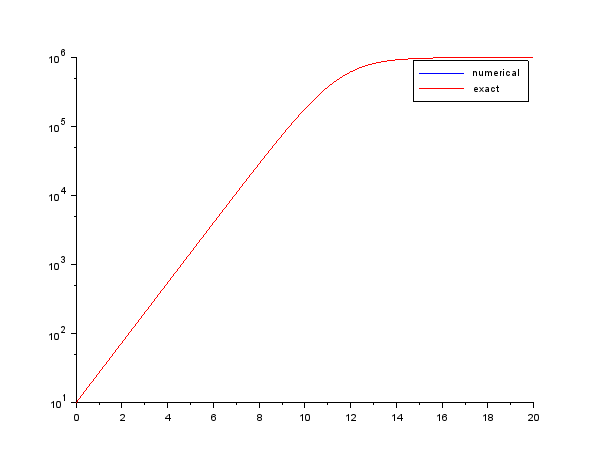
\includegraphics[width=0.5\textwidth,height=0.3\textwidth]{E1}
    \end{figure}
    Les deux images de fonction se chevauchent,On peut montrer que les solutions numériques et exactes de scilab sont très similaires\\
    ~\\
    Code pour cette question :
    \begin{verbatim}
        function ndot=f(t,n)
            ndot = 10^(-6) * n * (10^6 - n)
        endfunction

        n0=10;t0=0;B=10^(-6);n_infini=10^6
        t=0:0.1:20

        n=ode(n0,t0,t,f)
        plot2d("nl",t,n,style=2)

        function n_real=f_real(t)
            n_real=(n0.*n_infini.*exp(B.*n_infini.*t))./(n_infini-n0+n0.*exp(B.*n_infini.*t))
        endfunction

        plot2d("nl",t,f_real(t),style=5)
        legend("numerical","exact")
    \end{verbatim}
    

    \section*{Exercise 2: Duffing equation.}
    The Duffing differential equation
    \[\ddot{x}+\beta \dot{x}-x+\gamma x^3=Fcos(\omega t)\]
    can be written as a system of first-order differential equations as

    \begin{align*}
        \dot{x}&=v,\\
        \dot{v}&=-\beta v+x-\gamma x^3+Fcos(\omega t)
    \end{align*}
    
    Consider the function $F(t, x), x = (x_1, x_2)$ defined by
    $$
    F(t,x)=
    \begin{bmatrix}
        x_2\\
        -\beta x_2+x_1-\gamma x_1^3+Fcos(\omega t)
    \end{bmatrix}
    $$
    Write a Scilab function that implements F. Solve the Duffing equation by using the ode() solver of Scilab. For initial conditions and parameters, use $x_0 = (0, 0)^T , \beta = 0.05, \gamma = 1.0, \omega = 1.0, F = 6.0$ and the array of discrete times:
    \begin{verbatim}
        td = 0:0.05:200;
    \end{verbatim}
    Visualize the solution in the state space $(x1, x2)$ first, then as two time series $t\mapsto x_1(t), t\mapsto x_2(t)$.
    ~\\
    Solution :
    
    \begin{figure}[H]
        \centering
        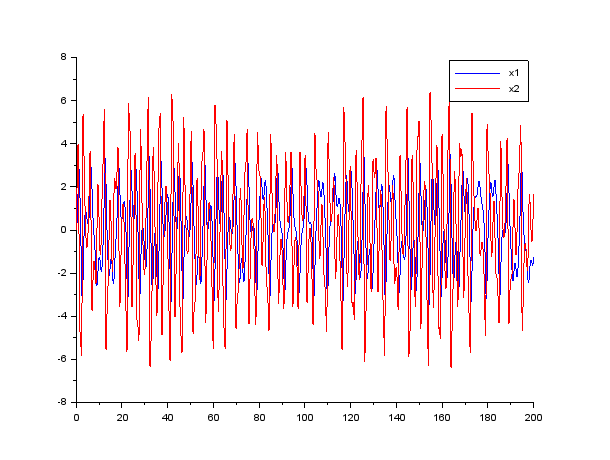
\includegraphics[width=0.8\textwidth,height=0.5\textwidth]{E2_2}
    \end{figure}
    
    \begin{figure}[H]
        \centering
        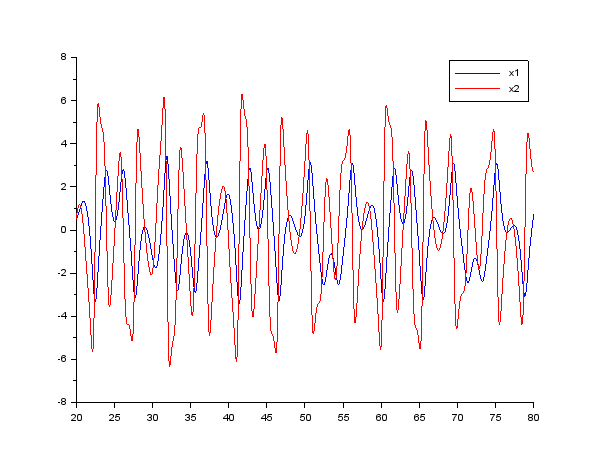
\includegraphics[width=0.8\textwidth,height=0.5\textwidth]{E2_3}
    \end{figure}
    ~\\
    Code pour cette question :
    \begin{verbatim}
        function E2=F2(t,x)
            E2(1) = x(2)
            E2(2) = -B.*x(2) + x(1) - yg.*x(1)^3 + F.*cos(w*t)
        endfunction

        B=0.05;yg=1.0;w=1.0;F=6.0;
        x0=[0;0]
        t0=0
        td=0:0.05:200

        E2=ode(x0,t0,td,F2)
        plot2d(td,E2(1,:),style=2,rect=[20,-8,80,8])
        plot2d(td,E2(2,:),style=5,rect=[20,-8,80,8])
        legend("x1","x2")
    \end{verbatim}


    \section*{Exercise 3: SEIRS Covid-19 differential model.}
    Consider the following Suspectible-Exposed-Infected-Recovered-susceptible virus outbreak model
    \begin{align*}
        \dot{S}(t)&=-\frac{\beta SI}{N} + \varepsilon R(1-R/N),\\
        \dot{E}(t)&=\frac{\beta SI}{N} -\sigma E,\\
        \dot{I}(t)&=\sigma E - \gamma I,\\
        \dot{R}(t)&=\gamma I - \varepsilon R(1-R/N)
    \end{align*}
    where$N=S+E+I+R$.\\
    For the numerical experiments, consider the following initial data $S(0)=70*10^6,E(0)=2000,I(0)=100,R(0)-0$ with parameters$\beta=1/2,\varepsilon=1/90,\sigma=1/5,\gamma=1/6$and a time window $t\in[0,700]$(days).\\
    use ode() of Scilab to compute the approximate solution of the differential problem. On the same grpahics, plot the respective time series $t\mapsto S(t),t\mapsto E(t),t\mapsto I(t),t\mapsto R(t)$. Try to interpret the behaviour of the solution.
    ~\\
    Solution :
    \begin{figure}[H]
        \centering
        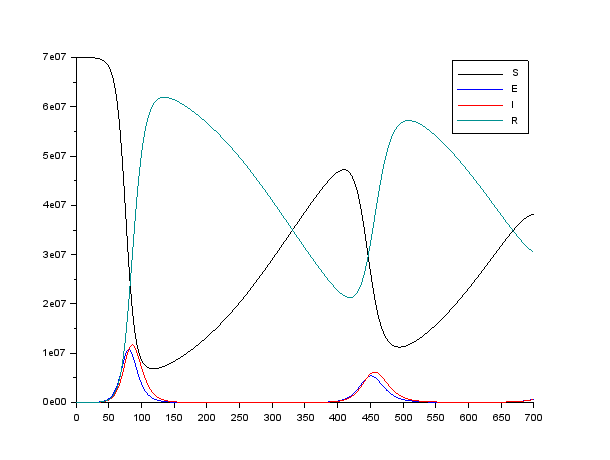
\includegraphics[width=0.8\textwidth,height=0.5\textwidth]{E3_1}
        \caption{modèle orginal}
    \end{figure}
    Nous observons la première épidémie de COVID :
    \begin{figure}[H]
        \centering
        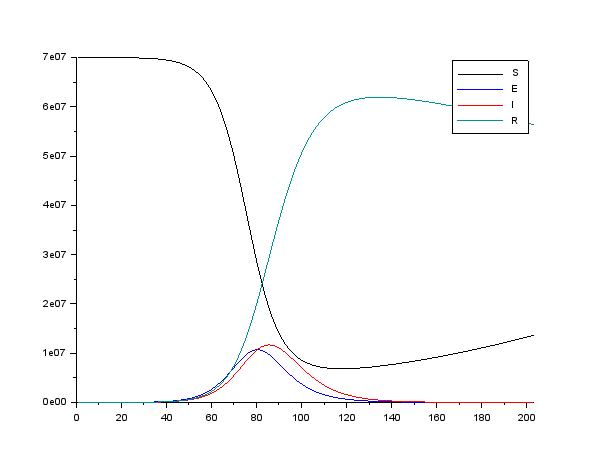
\includegraphics[width=0.8\textwidth,height=0.5\textwidth]{E3_2}
    \end{figure}
    En ajoutant le terme $\varepsilon R(1 - R/N )$, nous pouvons simuler la situation où le modèle sera effectivement infecté à nouveau après l'infection par le COVID.
    Cependant, le modèle peut encore être amélioré. Par exemple, il est possible qu'une personne en phase de E infecte une personne en phase de S, et si nous fixons la probabilité qu'une personne en phase de E infecte une personne normale à 1/5, le modèle devient la série d'équations suivante

    \begin{align*}
        \dot{S}(t)&=-\frac{\beta SI}{N} + \varepsilon R(1-R/N) -\frac{\beta_2SE}{N},\\
        \dot{E}(t)&=\frac{\beta SI}{N} -\sigma E + \frac{\beta_2SE}{N},\\
        \dot{I}(t)&=\sigma E - \gamma I,\\
        \dot{R}(t)&=\gamma I - \varepsilon R(1-R/N)
    \end{align*}
    \begin{figure}[H]
        \centering
        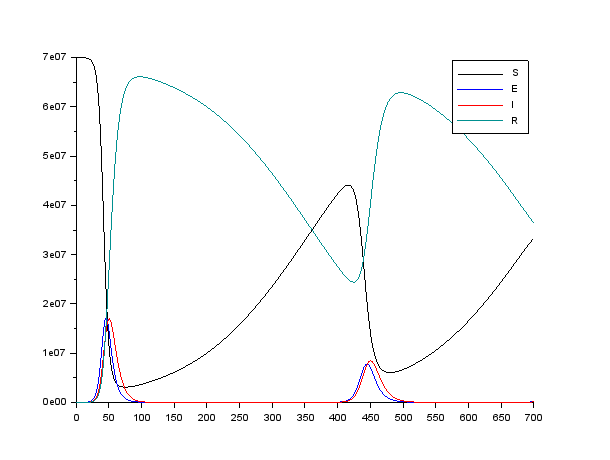
\includegraphics[width=0.8\textwidth,height=0.5\textwidth]{aaaa}
        \caption{modèle amélioré}
    \end{figure}
    Nous pouvons voir que cela avance le moment et la vitesse de l'apparition de l'infection. Dans le modèle original, le pic ne se produit que 90 jours après la fixation, alors que dans le modèle amélioré, le pic se produit à 50 jours.
    ~\\
    Code pour cette question :
    \begin{verbatim}
        function E3=F3(t,N)
            S=N(1);E=N(2);I=N(3);R=N(4)
            NN=S+E+I+R
            E3(1)=-(Beta.*S.*I)./(NN)+ varepsilon.*R.*(1-R./NN)
            E3(2)= (Beta.*S.*I)./(NN) - sigma.*E 
            E3(3)= sigma.*E - Gamma.*I
            E3(4)= Gamma.*I - varepsilon.*R.*(1-R./NN)
        endfunction

        function E3_2=F3_2(t,N)
            S=N(1);E=N(2);I=N(3);R=N(4)
            NN=S+E+I+R
            E3(1)=-(Beta.*S.*I)./(NN) + varepsilon.*R.*(1-R./NN) -Beta2*E*S./NN
            E3(2)= (Beta.*S.*I)./(NN) - sigma.*E + (Beta2*E*S./NN)
            E3(3)= sigma.*E - Gamma.*I
            E3(4)= Gamma.*I - varepsilon.*R.*(1-R./NN)
        endfunction

        S0=70*10^6;E0=2000;I0=100;R0=0
        Beta=1/2;varepsilon=1/90;sigma=1/5;Gamma=1/6;Beta2=1/5
        t0=0
        t=1:1:700
        N0=[S0;E0;I0;R0]

        E3=ode(N0,t0,t,F3)

        plot2d(t,E3(1,:))
        plot2d(t,E3(2,:),style=2)
        plot2d(t,E3(3,:),style=5)
        plot2d(t,E3(4,:),style=16)
        legend("S","E","I","R")
    \end{verbatim}
    \section*{Résumé}
    Lorsqu'on compose un modèle mathématique, on doit constamment améliorer son modèle en fonction de la situation réelle, mais le modèle lui-même a besoin d'un paramètre, et l'acquisition de ce paramètre nécessite des données réalistes.
\end{document}